\section{Stationary States}

\subsection{Introduction to Stationary States}\label{stationary_states}

We have now, after 51 pages, finally accumulated the necessary knowledge to begin solving quantum systems. But first, we must define what we are even trying to solve for.

In classical mechanics, we often wish to know the position $x(t)$ of a particle at a time $t$. The particle may be interacting with other particles or fields; we can represent these interactions by giving the particle some potential energy $V(x)$. 

In quantum mechanics, particles have indeterminate positions, so we cannot simply solve for some position function $x(t)$. Instead, we search for the \textit{state} of the particle, $\Psi(x,t)$. Often, in order to find the possible wavefunctions, we will also need to solve for the allowed energy values of quantum systems. 

For reasons that will soon become clear, we only care about \textbf{stationary states} of quantum systems. A stationary state has factorizable space and time dependence.

\begin{frameddefn}[Stationary state]
    A state $\Psi(x,t)$ is \textbf{stationary} if we can find $g(t)$ and $\psi(x)$ such that $$\Psi(x,t)=g(t)\psi(x).$$
\end{frameddefn}

Note that stationary states \textit{can} be time-dependent according to $g(t)$ above. The key property of stationary states is that the expectation values of observables with no explicit time dependence (like $x$) are time-independent.

We now reference Theorem \ref{general_schrodinger_eqn}, the general Schrödinger equation, which we rewrite for convenience: $$i\hbar\frac{\partial\Psi}{\partial t}=\bigg(-\frac{\hbar^2}{2m}\frac{\partial^2}{\partial x^2}+V(x)\bigg)\Psi=\hat{H}\Psi.$$We assume the potential $V$ is time-independent. If $\Psi$ is stationary, we have $$i\hbar\,\psi(x)\frac{dg(t)}{dt}=g(t)\hat{H}\psi(x),$$since $g(t)$ is unaffected by $\hat{H}$. Dividing by $\Psi(x,t)$, we have $$i\hbar\frac{1}{g(t)}\frac{dg(t)}{dt}=\frac{1}{\psi(x)}\hat{H}\psi(x).$$The left-hand side is a function of only time, while the right-hand side is a function of only space! We conclude that both sides must be equal to some constant $E$ with units of energy. Solving for $g(t)$, $$i\hbar\frac{dg(t)}{dt}=E\,g(t)\implies g(t)=Ce^{-\frac{iEt}{\hbar}}.$$Similarly, we have $$\hat{H}\psi=E\psi.$$This equation is an eigenvalue equation for the Hermitian operator $\hat{H}$, so stationary states are energy eigenfunctions. By Proposition \ref{9.1.2}, $E$ must be real.

Rewriting the left-hand side of the Schrödinger equation for a stationary state, we reach the \textbf{time-independent Schrödinger equation}:

\begin{framedthm}[Time-Independent Schrödinger Equation]\label{time-independent-schrodinger}
    $$\bigg(-\frac{\hbar^2}{2m}\frac{d^2}{dx^2}+V(x)\bigg)\psi(x)=E\,\psi(x).$$
\end{framedthm}

The general solutions can be written in the form $$\Psi(x,t)=C\psi(x)e^{-\frac{iEt}{\hbar}}.$$Now let's try to find the normalization condition. We have $$1=\int\Psi^*(x,t)\Psi(x,t)\,dx=\int dx\,\psi^*(x)e^{\frac{iEt}{\hbar}}\psi(x)e^{-\frac{iEt}{\hbar}}.$$Since $E$ is real, the two exponentials cancel, leaving $$\int dx\,\psi^*(x)\psi(x)=1.$$Thus, a stationary state is normalized if and only if the spatial component is normalized.

\subsection{Expectation Values in Stationary States}\label{expectation_stationary}

Consider the expectation value of the Hamiltonian on a stationary state $\Psi(x,t)$. We have that $$\langle\hat{H}\rangle_\Psi=\int dx\,\Psi^*\hat{H}\Psi=\int dx\,\psi^*(x)e^{\frac{iEt}{\hbar}}\hat{H}e^{-\frac{iEt}{\hbar}}\psi(x).$$Since the Hamiltonian does not affect the time-dependent terms, we have $$\langle\hat{H}\rangle_\Psi=\int dx\,\psi^*\hat{H}\psi=\langle\hat{H}\rangle_\psi.$$Thus, the expectation value of $\hat{H}$ in a stationary state is time-independent. We also know that $\hat{H}\psi=E\psi$, so $\langle\hat{H}\rangle_\Psi=E\int dx\,\psi^*\psi=E$. Since the stationary state is an eigenstate of $\hat{H}$, we see that the uncertainty $\Delta\hat{H}$ in $\Psi$ is $0$. In fact, this generalizes to \textit{any} time-independent operator $\hat{Q}$ -- the expectation value of $\hat{Q}$ on any stationary state is time-independent: $$\langle\hat{Q}\rangle_\Psi=\int dx\,\Psi^*\hat{Q}\Psi=\int dx\,\psi^*\hat{Q}\psi=\langle\hat{Q}\rangle_\psi.$$

\begin{framedrmk*}[Superposition of stationary states]
    An important observation is that the superposition of stationary states may not be stationary. This is because a state is stationary if we can factor out the time-dependence into some exponential term $e^{-\frac{iEt}{\hbar}}$. If we try to combine two stationary states with different values of $E$, we will no longer be able to factor out this term, so the resulting state will not be stationary, and so the expectation values of operators will be time-dependent. 

    In fact, given the superposition $\Psi(x,t)=c_1e^{-\frac{iE_1t}{\hbar}}\psi_1(x)+c_2e^{-\frac{iE_2t}{\hbar}}\psi_2(x)$, some very messy algebra yields $$\langle\hat{Q}\rangle_\Psi=|c_1|^2\langle\hat{Q}\rangle_{\psi_1}+|c_2|^2\langle\hat{Q}\rangle_{\psi_2}+2\text{Re}\bigg[c_1^*c_2e^{\frac{i(E_1-E_2)t}{\hbar}}(\psi_1,\hat{Q}\psi_2)\bigg].$$ Note that whenever $E_1\neq E_2$ and $(\psi_1,\hat{Q}\psi_2)\neq 0$, this expectation value is time-dependent.
\end{framedrmk*} 

\subsection{Spectrum and Continuity Conditions}\label{spectrum_continuity_conditions}

We now study the solutions to Theorem \ref{time-independent-schrodinger}: $$\hat{H}\psi(x)=E\psi(x).$$For a given Hamiltonian $\hat{H}$, we are interested in finding the eigenstates $\psi$ and the energy eigenvalues $E$. Generally, the possible values of $E$ are discrete, although they can also be continuous. Assuming they are discrete and countable, we can list the possible eigenstates \begin{align*}\psi_1&,\quad E_1\\\psi_2&,\quad E_2\\\vdots\ &\qquad\,\vdots\end{align*}This list is called the \textbf{spectrum} of the system. By Theorem \ref{spectral}, we can arrange these eigenstates into an orthonormal basis of the space of possible wavefunctions: $$(\psi_i,\psi_j)=\delta_{ij}.$$We can rewrite the time-independent Schrödinger Equation as $$\frac{d^2\psi}{dx^2}=\frac{2m}{\hbar}(V(x)-E)\psi.$$The possible solutions depend on the potential $V(x)$. Here, we consider the following types of potentials: 

\begin{itemize}
    \item Potentials that are continuous
    \item Potentials with a finite numbers of discontinuities
    \item Potentials that become infinity beyond certain points (i.e. potentials with a hard wall)
    \item Potentials containing delta functions
\end{itemize}

However, we do \textit{not} allow potentials that are worse than these cases --- for example, potentials containing powers or derivatives of delta functions.

We claim that $\psi(x)$ must be continuous. If it were not, there would be a jump, so $\psi'(x)$ would have to contain delta functions. Then $\psi''(x)$ would have to contain \textit{derivatives} of delta functions, which would require $V(x)$ to contain these. Also note that if $\psi'$ were discontinuous, then $\psi''$ would contain delta functions, so $V(x)$ would have to contain delta functions. 

\section{A Few Potentials}
\subsection{Solving Particle on a Circle}\label{solving_particle_on_circle}

In Section \ref{particle-on-a-circle}, we considered a particular wavefunction on a circle and found the possible values of momentum and their probabilities. We now solve for all the possible wavefunctions.

We represent the circle with circumference $L$ as the real line under the equivalence relation $x\sim x+L$. This implies that any wavefunction on a circle must satisfy the periodicity condition $\psi(x+L)=\psi(x)$. We also assume the particle is free, so $V(x)=0$. Then the time-independent Schrödinger Equation becomes $$-\frac{\hbar^2}{2m}\frac{d^2\psi}{dx^2}=E\psi.$$Before we solve this, we show that any solution must have $E\geq 0$. For this multiply both sides of the above equation by $\psi^*(x)$ and integrate over the circle:$$-\frac{\hbar^2}{2m}\int_0^L dx\,\psi^*(x)\frac{d}{dx}\frac{d}{dx}\psi(x)=E\int_0^L dx\,\psi^*\psi=E,$$assuming $\psi$ is normalized. We can rewrite the integral as follows: $$-\frac{\hbar^2}{2m}\int dx\,\bigg[\frac{d}{dx}(\psi^*\frac{d\psi}{dx})-\frac{d\psi^*}{dx}\frac{d\psi}{dx}\bigg]=E.$$We now split this into two terms: $$-\frac{\hbar^2}{2m}\psi^*\frac{d\psi}{dx}\bigg]_0^L+\frac{\hbar^2}{2m}\int_0^L dx\bigg|\frac{d\psi}{dx}\bigg|^2=E.$$Since $\psi$ and its derivatives are periodic, the first term is $0$. Thus, $E$ is the integral of a nonnegative quantity and thus must be nonnegative. We also see that $E=0$ requires $\psi$ to be constant.

Having shown that $E\geq 0$, we rewrite the Schrödinger Equation: $$\frac{d^2\psi}{dx^2}=-(\frac{2mE}{\hbar^2}\psi)=-k^2\psi,$$where $k^2=\frac{2mE}{\hbar^2}$, so $E=\frac{\hbar^2k^2}{2m}$. In other words, $k$ is still the wavenumber such that $p=\hbar k$. We are left with the familiar $$\frac{d^2\psi}{dx^2}=-k^2\psi.$$This is solved by sinusoidal functions: $\psi(x)\sim e^{ikx}$.

We now apply the periodicity condition: we must have $e^{ikx}=e^{ik(x+L)}$, which implies that $e^{ikL}=1$. Thus, $kL=2\pi n$ for some $n\in\mathbb{Z}$. We write $k_n=\frac{2\pi n}{L}$ to represent the value of $k$ corresponding to some $n$. Also, recall that the energy eigenvalue corresponding to some value of $k$ is given by $E_n=\frac{\hbar^2k_n^2}{2m}=\frac{2\pi^2\hbar^2n^2}{mL^2}$. The eigenstate with this eigenvalue is given by $\psi_n(x)=Ne^{ik_nx}$ for some normalization constant $N$, which we can compute as follows: $$\int_0^L|Ne^{ik_nx}|^2\,dx=\int_0^L N^2=N^2L=1,$$from which we conclude $N=\frac{1}{\sqrt{L}}$. Thus the energy eigenstates are $$\boxed{\psi_n(x)=\frac{1}{\sqrt{L}}e^{ik_nx}=\frac{1}{\sqrt{L}}e^{2\pi inx/L}}$$The full stationary states have an $e^{-iE_nt/\hbar}$ time dependence. Note that $E_n=E_{-n}$ for all $n\in\mathbb{Z}$; thus, we have degenerate states. In fact, the only non-degenerate eigenstate is $\psi_0=\frac{1}{\sqrt{L}}$. 

Whenever we find degenerate eigenstates, we must wonder what physical property distinguishes them. That is, we wish to find an observable that takes on different values in those states. In this case, the answer is momentum: $\psi_n(x)$ has momentum $p_n=\hbar k_n=2\pi n\frac{\hbar}{L}$ while $\psi_{-n}(x)$ has momentum $-2\pi n\frac{\hbar}{L}$.\footnote{These states can be thought of as representing waves with the same frequency propagating clockwise and counter-clockwise around the circle, respectively.}

Consider the degenerate eigenstates $\psi_n$ and $\psi_{-n}$. Then any linear combination of them is also an eigenstate with eigenvalue $E_n$, including $\psi_n+\psi_{-n}\sim \cos k_nx$, and $\psi_n-\psi_{-n}\sim\sin k_nx$. However, these are no longer momentum eigenstates. Only our exponentials $\psi_n$ are simultaneous eigenstates of both energy and momentum.

Since the energy eigenstates are also momentum eigenstates with no degeneracies, they are automatically orthonormal by Proposition \ref{9.2.1}. By Theorem \ref{spectral}, any wavefunction $\psi(x)$ satisfying the periodicity condition can be written as $$\psi(x)=\sum_{n\in\mathbb{Z}}a_n\psi_n(x),$$where the coefficients $a_n$ can be determined by the integrals $$a_n=\int_0^L dx\,\psi_n^*(x)\Psi(x,0).$$

\subsection{The Infinite Square Well}\label{infinite_square_well}

We now introduce another instructive toy model, the \textbf{infinite square well} $$V(x)=
\begin{cases} 
      0 & 0<x<a \\
      \infty & x\leq 0,\,x\geq a\\
   \end{cases}$$The infinite potential outside the well $(0,a)$ makes the wavefunction vanish outside this region: a particle outside these bounds would have to have infinite energy. As we will see later, particles \textit{can} be found outside \textit{finite} square wells in quantum mechanics, but not infinite ones.
   
We conclude that $\psi(x)=0$ for all $x<0$ and $x>a$. Since the wavefunction must be continuous, it should also vanish at $x=0$ and $x=a$. These are the \textit{boundary conditions}.

\begin{framedrmk*}[Discontinuous derivative]
    You may wonder about the continuity of the first derivative $\psi'(x)$. This derivative vanishes outside the well and continuity would say that $\psi'$ should vanish at $x=0$ and $x=a$. But a solution to the Schrödinger equation (a second-order differential equation) where both the wavefunction and its derivative vanish at a point is constant and zero! If a solution exists, therefore, we must accept that $\psi'(x)$ can have discontinuities at the boundaries of the well.
\end{framedrmk*}

As before, the Schrödinger equation can be written as $\psi''=-k^2\psi(x)$ for $k^2=\frac{2mE}{\hbar^2}$. The general solution can then be written as $\psi(x)=c_1\cos kx+c_2\sin kx$. However, note that $\psi(0)=c_1=0$ by the first boundary condition! We are left with possible solutions of the form $$\psi(x)=c_2\sin kx.$$We also know that $\psi(a)=c_2\sin ka=0$, and since $c_2\neq 0$ (in which case there would simply be no particle in the well), we have $ka=n\pi$ for $n\in\mathbb{Z}$.\footnote{Note that this is the same condition for standing waves on a string, and as a result the stationary states are standing waves.} Let $k_n=\frac{\pi n}{a}$ be the value of $k$ associated with the integer $n$. Our solutions would be $$\psi_n(x)=N\sin(\frac{n\pi x}{a}).$$This time, we cannot take all integers $n$. First of all, $k_0=0$, so $\psi_0=c_2\sin k_0x$ is zero at all points, which is not allowed. Furthermore, $\psi_n$ and $\psi_{-n}$ are identical up to a sign, which has no physical significance. \footnote{Recall that for the particle on a circle, the wavefunctions for $k_n$ and $k_{-n}$ \textit{were} physically different: they produced different momentum eigenvalues.} Thus, we restrict $n\in\mathbb{N}$. 

We find the normalization constant $N$ by taking $$\int_0^a|\psi_n|^2\,dx=N^2\int_0^a dx\,\sin^2(\frac{n\pi x}{a}).$$Since the interval of integration contains an integer number of half-periods of $\sin^2(x)$, the argument averages to $\frac{1}{2}$. Thus, $$\int_0^a|\psi_n|^2\,dx=\frac{N^2}{2a}=1,$$so $N=\sqrt{\frac{2}{a}}$. The energy eigenstates can thus be written as $$\boxed{\psi_n(x)=\sqrt{\frac{2}{a}}\sin(\frac{n\pi x}{a})}$$for $n\in\mathbb{N}$ with $E_n=\frac{\hbar^2\pi^2n^2}{2ma^2}$. We call the minimum energy state $\psi_1$ the \textbf{ground state}. Higher energy states are called \textbf{excited states}. Since $n$ is restricted to positive values, there are no degeneracies.

\begin{frameddefn}[Bound states]
    A state $\Psi$ in a 1-dimensional potential is a \textbf{bound state} if it is normalizable. This implies that $\Psi$ must go to $0$ at $x=\pm\infty$. Clearly, all eigenstates of the infinite square well are bound states.
\end{frameddefn}

\subsection{Nodes and Symmetries in the Infinite Square Well}\label{nodes_and_symmetries_infinite_square_well}

Figure \ref{infinite_square_well_graph} shows a graph of the four lowest energy eigenstates for an infinite square well centered about the origin. We state several facts about the eigenstates of the infinite square well that we will later generalize to other $1$-dimensional potentials.

\begin{figure}[H]
    \centering
    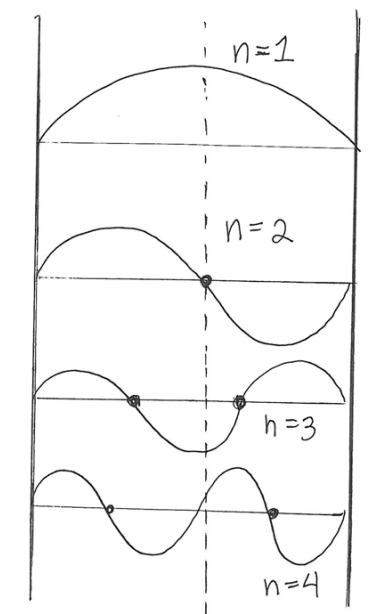
\includegraphics[width=0.5\linewidth]{resources/images/infinite_square_well_eigenstates.png}
    \caption{Graphs of the first four energy eigenstates of the infinite square well centered at $x=0$.}
    \label{infinite_square_well_graph}
\end{figure}

We define a \textbf{node} to be a zero of the wavefunction that is not at an endpoint. Note that the ground state has no nodes. In fact, it is true that any normalizable ground state of a bounded one-dimensional potential has no nodes. Additionally, the $n$th solution $\psi_n$ has $n-1$ nodes. \footnote{See Theorem \ref{node_theorem}.} 

Notice from Figure \ref{infinite_square_well_graph} that the eigenstates alternate even and odd. This is also a general fact: bound states of a symmetric potential $V(x)=V(-x)$ are either odd or even.\footnote{See Corollary \ref{even_potential_cor}.}

Furthermore, we show that all one-dimensional bound states are non-degenerate in energy. Note that this was violated by the particle on a circle because those eigenstates were not bound: the particle was free to traverse the entire real line.

\begin{framedthm}[Non-degeneracy of bound states]\label{non-degeneracy_of_bound_states}
    In any one-dimensional potential $V(x)$, all bound states are non-degenerate in energy.

    \begin{proof}
        Suppose there exist bound states $\psi_1$ and $\psi_2$, both with energy $E$, in the potential $V(x)$. We show that $\psi_1$ and $\psi_2$ must then represent the same state. We have \begin{align*}
            \psi_1''+\frac{2m}{\hbar^2}(E-V)\psi_1&=0\\ \psi_2''+\frac{2m}{\hbar^2}(E-V)\psi_2 &= 0
        \end{align*} 
        Multiplying the first equation by $\psi_2$ and the second by $\psi_1$, 
        \begin{align*}
            \psi_1''\psi_2+\frac{2m}{\hbar^2}(E-V)\psi_1\psi_2&=0\\ \psi_2''\psi_1+\frac{2m}{\hbar^2}(E-V)\psi_2\psi_1 &= 0
        \end{align*} 
        Subtracting the second equation from the first, we have $$\psi_1''\psi_2-\psi_2''\psi_1=0.$$
        By integration by parts, $\int\psi_1''\psi_2=\psi_1'\psi_2-\int\psi_1'\psi_2'$, while $\int\psi_2''\psi_1=\psi_2'\psi_1-\int\psi_2'\psi_1'$. Integrating the above equation\footnote{This integration is possible because $\psi_1$ and $\psi_2$ are bound states, so their integrals do not diverge.} then gives $$\psi_1'\psi_2-\psi_1\psi_2'=0.$$Now recall that from the quotient rule, $$\frac{d}{dx}\bigg(\frac{\psi_1}{\psi_2}\bigg)=\frac{\psi_1'\psi_2-\psi_1\psi_2'}{\psi_2^2}.$$Since we know $\psi_1'\psi_2-\psi_1\psi_2'=0$, we conclude that $\frac{d}{dx}(\frac{\psi_1}{\psi_2})=0$, which implies that $\psi_1=C\psi_2$ for some constant $C$. But then $\psi_1$ and $\psi_2$ are the same state! We conclude that no degenerate bound states exist in one-dimensional potentials.
    \end{proof}
\end{framedthm}

\begin{framedrmk*}
    You might wonder what happens in two or three dimensions. It turns out that degeneracies become incredibly common! You can intuit this by thinking about energy in the classical sense. A one-dimensional particle with a given energy can only behave in one way. However, a two-dimensional particle with a given energy can move in infinitely different ways, depending on the $x$ and $y$ components of its velocity. A similar reasoning applies for quantum mechanical particles constrained to two-dimensional wells.
\end{framedrmk*}

\subsection{The Finite Square Well}\label{finite_square_well}

We next consider the \textbf{finite square well} of height $V_0$ and width $2a$: $$V(x)=
\begin{cases} 
      -V_0 & |x|<a \\
      0& |x|\geq a\\
   \end{cases}$$We will look for bound states, which must have energy $-V_0<E<0$. Otherwise, there would be plane waves propagating infinitely outside the well. For a bound state with energy $E$, the energy $\tilde{E}$ measured from the bottom of the potential is $\tilde{E}=V_0-|E|>0$; these $\tilde{E}$ can be compared with the energies of the infinite square well in the limit as $V_0$ goes to $\infty$.

The time-independent Schrödinger Equation for the finite square well is $$\psi''=\frac{-2m}{\hbar^2}(E-V(x))\psi.$$Let $\alpha(x)=\frac{-2m}{\hbar^2}(E-V(x))$. We consider the two regions separately.

\begin{itemize}
    \item If $|x|\geq a$, $\alpha(x)=\frac{-2m}{\hbar^2}E$ is a positive constant. In this region, the wavefunction is constructed with real exponentials.
    \item If $|x|<a$, $\alpha(x)=\frac{-2m}{\hbar^2}(V_0-|E|)$ is a negative constant. In this region, the wavefunction is constructed with trigonometric functions.
\end{itemize}

We now solve for the energy eigenstates. Note that $V(x)$ is symmetric, and by Corollary \ref{even_potential_cor}, all the bound states must be either odd or even. We deal with these cases separately.

\textbf{Even solutions.} We have $\psi(-x)=\psi(x)$. For $|x|<a$, we have $\psi''=\frac{-2m}{\hbar^2}(V_0-|E|)\psi$. We let $k^2=\frac{2m}{\hbar^2}(V_0-|E|)$, so that $$\psi''=-k^2\psi.$$Since $\psi$ must be even, the solutions are of the form $\psi(x)=\cos kx$, $|x|<a$.

\begin{framedrmk*}[Normalization constants]
    We do not include a normalization constant because we are looking for the possible energy eigenvalues $E$. As long as the wavefunctions are \textit{normalizable}, we do not care what the actual normalization constants are.
\end{framedrmk*}

For $|x|\geq a$, we have $\psi''=\frac{-2m}{\hbar^2}\psi=\frac{2m|E|}{\hbar^2}\psi$. We let $\kappa^2=\frac{2m|E|}{\hbar^2}$, so that $$\psi''=\kappa^2\psi.$$The solutions are of the form $\psi(x)=Ae^{-\kappa x}$, $x\geq a$ (the same thing is mirrored for negative $x$). Note that this time, we do need a normalization constant $A$, in order to ensure we can match the boundary conditions at $x=a$. 

Notice that $k^2$ and $\kappa^2$ satisfy the nice relation $k^2+\kappa^2=\frac{2mV_0}{\hbar^2}$. At this point, we make progress by defining a few unit-free constants.
\begin{align*}\eta&=k a>0,\\ \xi&=\kappa a>0,\\ z_0^2 &=\eta^2+\xi^2=\frac{2mV_0a^2}{\hbar^2}.\end{align*}We are left with a constant $z_0$ that depends on the properties of the potential. A deep, wide potential has large $z_0$, while a shallow, narrow potential has small $z_0$. Importantly, we will see that $z_0$ determines the number of bound states the square well has.

We can also solve for the relations $\frac{|E|}{V_0}=(\frac{\xi}{z_0})^2$ and $\tilde{E}=V_0-|E|=\eta^2\frac{\hbar^2}{2ma^2}$. The first equation gives the energy as a fraction of the depth of the well, while the second equation shows the similarity between the finite well and the infinite well, where the energy states were $E_n=\frac{\hbar^2\pi^2n^2}{2ma^2}$.

The condition that $\psi$ is continuous at $x=a$ yields $$\cos ka=Ae^{-\kappa a}.$$Furthermore, $\psi'$ must be continuous at $x=a$ since $V(x)$ contains no delta functions (See Section \ref{spectrum_continuity_conditions}).  This yields $$-k\sin ka=-\kappa Ae^{-\kappa a}.$$Dividing the second equation by the first gives $k\tan ka=\kappa.$ Multiplying both sides by $a$ to get rid of the units, $$\xi=\eta\tan\eta.$$Finding the even bound states is thus reduced to finding solutions to the equations $\eta^2+\xi^2=z_0^2$ and $\xi=\eta\tan\eta$, where $\eta$ and $\xi$ are both positive. 

The first equation is simply a quarter-circle with radius $r_0$. The second equation is similar in shape to the tangent function. Figure \ref{even_finite_square_well} shows these equations graphed together.

\begin{figure}[H]
    \centering
    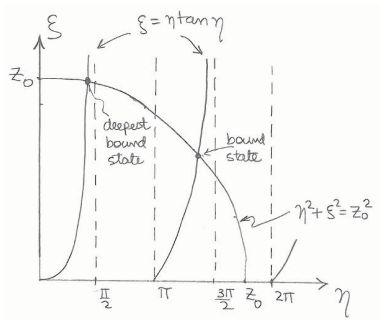
\includegraphics[width=0.5\linewidth]{resources/images/even_finite_square_well.png}
    \caption{A graph of the equations governing the even bound states of the finite square well.}
    \label{even_finite_square_well}
\end{figure}

Since we have $\frac{|E|}{V_0}=(\frac{\xi}{z_0})^2$, the deepest bound state, or the ground state, is the one with the largest $\xi$-coordinate. Note that as $z_0$ grows, it intersects more of the segments of $\xi=\eta\tan\eta$, so that there are more bound states. On the other hand, no matter how small $z_0$ is, there will always be at least one intersection point, representing the existence of at least one bound state

\textbf{Odd solutions.} For odd solutions, keeping all the definitions from above, we have $$\psi(x)=\begin{cases}\sin kx&|x|<a\\Ae^{-k|x|}&|x|>a\end{cases}$$The boundary conditions now give $\xi=-\eta\cot\eta$, and we keep the equation of the circle $\eta^2+\xi^2=z_0^2$. Plotting these curves together, we get Figure \ref{odd_finite_square_well}.

\begin{figure}[H]
    \centering
    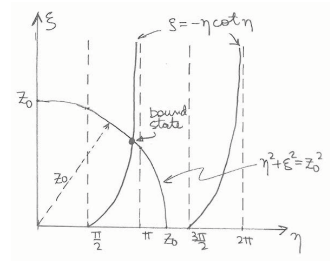
\includegraphics[width=0.5\linewidth]{resources/images/odd_finite_square_well.png}
    \caption{A graph of the equations governing the odd bound states of the finite square well.}
    \label{odd_finite_square_well}
\end{figure}

Note that the curve $\xi=-\eta\cot\eta$ is negative for $\eta<\pi/2$ and thus does not appear in this region. For $z_0<\frac{\pi}{2}$, there are no odd bound state solutions.

Sketches of the first three eigenstates of the finite square well are shown in Figure \ref{finite_well_eigenstates}. They alternate even and odd, and they have successively more nodes.

\begin{figure}
    \centering
    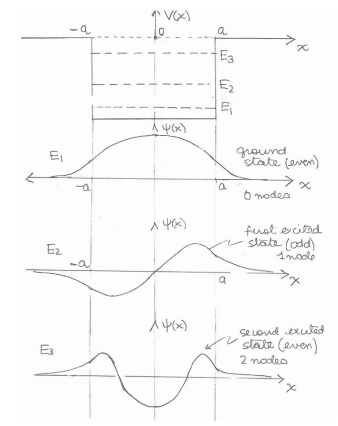
\includegraphics[width=0.5\linewidth]{resources/images/finite_well_eigenstates.png}
    \caption{Sketches of the first three eigenstates of the finite square well.}
    \label{finite_well_eigenstates}
\end{figure}